\chapter{Métodos numéricos}\label{capitulo:metodos_numericos}

A integração numérica é o processo de aproximar o valor de uma integral numericamente com alguma margem de erro. Existe uma infinidade de formas de calcular essa aproximação, desde métodos baseados puramente em ferramentas básicas de cálculo até métodos baseados em teoria de variedades diferenciáveis e grupos de Lie.

Neste capítulo apresentamos uma pequena parte destes métodos, aplicando-os especificamente para a integração temporal, e contemplando principalmente o que foi utilizado nas simulações do PNCG. O capítulo começa com métodos tradicionais, baseados em cálculo de derivadas e geometria, principalmente para facilitar a habituação com os conceitos de integração numérica. Recomendamos \cite{alexandre_megiorin_roma_metodos_nodate} e \cite{Butcher2016-jx} para um estudo mais aprofundado.

Em seguida, entramos no ramo dos integradores simpléticos, aplicando numericamente os conceitos apresentados no capítulo \ref{capitulo:revisao_mecanica} a respeito da Mecânica Hamiltoniana. Em resumo, os integradores simpléticos são elaborados levando-se em conta não somente aspectos geométricos da função que está sendo integrada, mas também de todo o espaço que a contém. No caso, integramos sistemas hamiltonianos e portanto as propriedades do espaço de fases, como as integrais primeiras, são levadas em conta nos métodos através do conceito de \textit{simplectomorfismo}. A bibliografia principal utilizada e altamente recomendada é \cite{Hairer2006-oz} e \cite{Leimkuhler2005}.

Ao final, apresentamos um corretor numérico utilizado posteriormente à integração. O corretor se baseia nas integrais primeiras e aplica uma projeção via método de quadrados mínimos entre as hipersuperfícies no espaço de fases, fornecendo uma aproximação verossímil ao problema no sentido de que a estrutura simplética passa a ser conservada nas trajetórias ainda que não seja utilizado um integrador simplético.

Existem muitos outras formas de fazer a integração numérica. Em muitos contextos são utilizados métodos implícitos (explicados mais adiante), métodos com tamanho de passo variável, e até métodos voltados especificamente para o PNCG que preservam a energia e o momento angular com precisão de máquina, como \cite{Kotovych2002} propõem. Neste trabalho nos limitamos aos métodos explícitos tradicionais e aos simpléticos.

Por fim, os métodos foram testados com problemas-modelo escolhidos. Estes constam no Anexo \ref{apendice:problemas-modelo}.

% \begin{table}[]
%     \centering
%     \begin{tabular}{c|ccccccc}
%         $h$              & E. S. & Verlet & Ruth3 & Ruth4 & RK4 & RKN551 & RKN671  \\
%         \hline
%         $1/10$  & $1.129548$ & $1.904978$ & $3.567326$ & $3.398327$ &	$3.964893$ & $5.367215$ & $5.392546$ \\
%         $1/20$  & $1.057072$ & $1.974542$ & $3.659927$ & $3.840014$ &	$4.046272$ & $5.869322$ & $5.836890$ \\
%         $1/40$  & $1.021997$ & $1.993517$ & $3.540536$ & $3.959375$ &	$4.041771$ & $5.998531$ & $5.958402$ \\
%         $1/80$  & $1.008801$ & $1.998372$ & $3.361093$ & $3.989805$ &	$4.025951$ & $5.948801$ & $5.989673$ \\
%         $1/160$ & $1.003795$ & $1.999592$ & $3.208686$ & $3.997449$ &	$4.014280$ & $5.588236$ & $6.003132$ \\
%     \end{tabular}
%     \caption{Convergência dos métodos no problema modelo.}
%     \label{tab:my_label}
% \end{table}

% \begin{table}[]
%     \centering
%     \begin{tabular}{c|ccccc}
%         $h$              & E. E. & E. I. & RK22 & RK33 & RK44 \\
%         \hline
%         $1/40$   & $0.712071$ & $1.859924$ & $1.989241$ & $2.936490$ & $4.041771$ \\
%         $1/80$   & $0.827102$ & $1.283719$ & $2.003212$ & $2.965188$ & $4.025951$ \\
%         $1/160$  & $0.904085$ & $1.122329$ & $2.003873$ & $2.981701$ & $4.014280$ \\
%         $1/320$  & $0.949289$ & $1.057240$ & $2.002516$ & $2.990612$ & $4.008214$ \\
%         $1/640$  & $0.973898$ & $1.027730$ & $2.001404$ & $2.995243$ & $3.992159$ \\
%     \end{tabular}
%     \caption{Convergência dos métodos no problema modelo.}
%     \label{tab:my_label}
% \end{table}


%%%%%%%%%%%%%%%%%%%%%%%%%%%%%%%%%%%%%%%
%%% INTRODUÇÃO
%   Apresentar ideia dos métodos numéricos e a necessidade 
%   no caso do Problema de N-corpos. Falar brevemente dos 
%   tipos de métodos e o objetivo deste capítulo;
%%%%%%%%%%%%%%%%%%%%%%%%%%%%%%%%%%%%%%%
%%%%%%%%%%%%%%%%%%%%%%%%%%%%%%%%%%%%%%%%%%%%%%%%%%%%%%%%%%%%%%%%%
% > CONCEITOS BASICOS DE INTEGRACAO NUMERICA
%%%%%%%%%%%%%%%%%%%%%%%%%%%%%%%%%%%%%%%%%%%%%%%%%%%%%%%%%%%%%%%%%
\section{Conceitos básicos de integração numérica}

A ideia dos integradores numéricos é aproximar a solução exata de um problema de Cauchy em um intervalo $[a,b] \subseteq \R$, discretizando-o em um conjunto finito de $m+1$ pontos na forma
\begin{equation*}
    t_0 = a, \quad
    t_1 = t_0 + h_1 \quad
    \hdots \quad
    t_m = t_{m-1} + h_m = b,
\end{equation*}
onde cada $h_i \in \R$, $i = 1, ..., m$, é um \textit{passo de integração do instante $i$}. Neste trabalho, exceto quando explicitado o contrário, $h_i = h = (b-a)/m$, para todo $i$, então a discretização assume a forma
\begin{equation*}
    t_k = a + hk, \quad k = 1, 2, ..., m.
\end{equation*}

Com o intervalo discretizado, é possível obter uma diversidade de discretizações do problema em si. Assim, um problema do tipo
\begin{equation}\label{eq:problema_de_cauchy}
    \begin{cases}
        \der{}{t} y(t) = f(t,y(t)), \quad t \in [a,b], \\
        y(t_0) = y(a) = y_0,
    \end{cases}
\end{equation}
com $f:[a,b] \times \R^n \to \R^n$ e $y$ com condições suficientes para garantir existência e unicidade em $[a,b]$, pode ser discretizado na forma:
\begin{equation*}
    y(t_{k+1}) \approx y_{k+1} = \Phi_h(t_k, y_k), \quad k = 0, 1, ..., m-1,
\end{equation*}
onde $\Phi_h$ é chamado \textit{fluxo numérico} ou \textit{discreto}. Quando depender somente de $h$, $t_k$ e $y_k$, diremos que $\Phi_h$ é um \textit{método de passo único}; no caso contrário, será um \textit{método de passo múltiplo}.

Para cada instante da aproximação, podemos definir um \textit{erro local de discretização}.

\begin{definition}\label{def:erro_local_discretizacao}
    O \textbf{erro local de discretização} $\alpha_k$ do método numérico $\Phi_h$ em um instante discretizado $t_k \in [a,b]$ é dado por:
    \begin{equation*}
        \alpha_k := \dfrac{y(t_{k+1}) - \Phi_h(t_k, y(t_k))}{h}.
    \end{equation*}
\end{definition}

Nesse sentido, suponha que $\Phi_h$ é um método de passo único, ou seja, $\Phi_h(t_k,y_k) = y_k + h \tilde{\Phi}_h(t_k,y_k)$. Pensando na integração de Riemann, é intuitivo que quanto menor o tamanho de $h$, menor também será o erro. Porém, se $h \to 0$, uma vez que $t_k = h k + t_0$, teria-se que $t_k = t_0$ sempre. A saída para isso é fixar $t \in [a,b]$ e manter $hk = t - t_0$ fixo com $h \to 0$, o que significa que $k \to \infty$. Temos então para o erro local:
\begin{align*}
    \lim_{h \to 0} \alpha_k
    &= \lim_{h \to 0} \left[ \dfrac{y(t_{k+1}) - \Phi_h(t_k, y(t_k))}{h} \right] \\
    &= \lim_{h \to 0} \left[ \dfrac{y(t_k + h) - y(t_k)}{h} - \tilde{\Phi}_h(t_k, y_k) \right] \\
    &= f(t,y(t)) - \tilde{\Phi}_0(t,y(t)).
\end{align*}

Para um problema bem posto, espera-se de um método numérico então que o erro local deva ser cada vez menor, e que no limite seja zero. Nesse caso, dizemos que o método é \textit{consistente}.

\begin{definition}
    Dizemos que um integrador de passo único $\Phi_h(t_k,y_k) = y_k + h \tilde{\Phi}_h(t_k,y_k)$ é \textbf{consistente} se $\tilde{\Phi}_0(t,y) = f(t,y)$ ou, equivalentemente, $\lim_{h \to 0} \alpha_k = 0$, para $t \in [a,b]$ com $hk = t - t_0$ fixado.
\end{definition}

A consistência garante que, em alguma medida, a aproximação fornecida pelo método numérico (a partir de um valor exato e conhecido da trajetória) é próxima da solução exata do problema. Assim, também é possível atribuir à consistência uma \textit{ordem} da maneira que segue.

\begin{definition}
    Se existirem $C, h_0, q >0$ para quaisquer $h$ e $k$, tais que o erro local satisfaça:
    \begin{equation*}
        \max_k \norma{\alpha_k} \leq C h^q, \quad 0 < h \leq h_0,
    \end{equation*}
    então o método tem \textit{ordem de consistência} $q$ atrelada a norma $\norma{\cdot}$, que, a menos da explicitação do contrário, será a norma euclidiana usual.
    Nesse caso, um método consistente com ordem de consistência $q$ pode ser escrito da seguinte maneira:
    \begin{equation*}
        y(t_{k+1}) = \Phi_h(t_k, y_k) + O(h^q).
    \end{equation*}
\end{definition}

O que ocorre, porém, é que no geral se conhece somente o valor inicial do problema, e então define-se outra medida de erro, chamada \textit{erro global}. 

\begin{definition}
    O erro global $e_h(t_k)$ é o erro acumulado pelo método numérico até o instante discreto $t_k$:
    \begin{equation*}
        e_h (t_k) := e_k := y(t_k) - y_k.
    \end{equation*}
\end{definition}

O que se espera de um método minimamente utilizável é que seu erro global esteja ligado somente com o tamanho do passo $h$, de modo que 
\begin{equation}\label{eq:criterio_convergencia_1}
    \lim_{h \to 0} \dfrac{e_k}{h} = 0, \quad k = 0, 1, ..., m-1.
\end{equation}
para qualquer problema de Cauchy bem posto. 

\begin{definition}\label{def:convergencia}
    Um integrador $\Phi_h$ para o qual vale \ref{eq:criterio_convergencia_1} para qualquer problema de Cauchy bem posto é dito \textbf{convergente}, e dizemos que o integrador de passo único e explícito tem ordem de convergência $p$ se, e só se,
    \begin{equation*}
        e_h(t) = O(h^{p+1}).
    \end{equation*}
\end{definition}

A partir do erro global, é possível determinar condições suficientes para que um método de passo único explícito seja convergente. Supondo que $\tilde{\Phi}_h (t_k, \vet y_k) = \dfrac{1}{h} (\Phi_h (t_k, \vet y_k) - \vet y_k)$ satisfaça a condição de Lipschitz para $\vet y$, ou seja,
\begin{equation*}
    \norma{\tilde{\Phi}_h(t, \vet y_1) - \tilde{\Phi}_h(t, \vet y_2)}
    \leq
    L \norma{\vet y_1 - \vet y_2}
\end{equation*}
e que o erro de discretização local $\alpha_k$ seja limitado por $\alpha$, então \citep[29]{alexandre_megiorin_roma_metodos_nodate}
\begin{equation}
    \norma{e_k} \leq e^{k h L} \norma{e_0} + \dfrac{e^{k h L} - 1}{L} \alpha.
\end{equation}

Para o que interessa neste trabalho, $\norma{e_0} = 0$, então se um método explícito e de passo único é consistente com ordem $q$, ou seja, existe $C$ constante tal que $\alpha = C h^q$, então
\begin{equation*}
    \norma{e_k} \leq \dfrac{e^{k h L} - 1}{L} C h^q.
\end{equation*}
Dessa forma, o método também é convergente de ordem $q$.

Através do erro global, também é possível obter uma expansão em série de potências para uma aproximação numérica. Trataremos a questão para problemas de Cauchy em $\R$ por maior facilidade de exposição, mas todo o processo pode ser estendido para mais dimensões aplicando normas sobre os vetores.

\begin{theorem}\label{teorema:erro_global_expansao}\citep[30]{alexandre_megiorin_roma_metodos_nodate}
    Considere um problema de Cauchy com solução suficientemente diferenciável em um intervalo $[a,b]$ e uma aproximação $\eta(t,h)$ obtida através de um método de passo único
    \begin{equation*}
        \eta_{k+1} = \eta_k + h \tilde \Phi(t_k, \eta_k, h)
    \end{equation*}
    de ordem $p$ com tamanho de passo fixo $h = (t-t_0)/n$ para cada $t_0, t \in [a,b]$ e $n$ inteiro positivo. Nessas condições, $\eta(t,h)$ admite expansão em potências de $h$ da forma
    \begin{equation*}
        \eta(t,h) = y(t) + h^p e_p (t) + h^{p+1} e_{p+1} (t) + \hdots + h^N e_N(t) + h^{N+1} E_{N+1}(t,h).
    \end{equation*}
\end{theorem}

Do teorema \ref{teorema:erro_global_expansao} decorre que o erro de discretização global no instante $t$ pode ser escrito como
\begin{equation*}
    - e_h (t) = \eta (t,h) - y(t) = \sum_{j=p}^N h^j e_j(t) + h^{N+1} E_{N+1} (t,h).
\end{equation*}
Nesse sentido, para um $h$ suficientemente pequeno, temos uma aproximação razoável para o erro:
\begin{equation*}
    - e_h (t) = \eta (t, h) - y(t) \approx e_p (t) h^p.
\end{equation*}
Observe que a diferença entre aproximações com tamanho de passo $h$ e $h/2$ pode ser aproximado por
\begin{equation*}
    \eta (t, h) - \eta(t, h/2) \approx e_p(t) \left(\dfrac{h}{2}\right)^p (2^p - 1)
\end{equation*}
e logo
\begin{equation*}
    e_p (t) \left(\dfrac{h}{2}\right)^p \approx \dfrac{\eta (t, h) - \eta (t,h/2)}{2^p - 1}.
\end{equation*}
Isso fornece um valor aproximado para $e_{h/2}(t)$ se considerando um $h > 0$ suficientemente pequeno:
\begin{equation*}
    e_{h/2} (t) \approx - \dfrac{\eta(t,h) - \eta(t,h/2)}{2^p -  1}.
\end{equation*}

Todo esse processo supõe que o valor de $p$ é conhecido. No entanto, para fins práticos, é possível estimar $p$ realizando simulações com diferentes tamanhos de passo. Para um tamanho de passo $h$ de referência, considere $\eta (t, 2h)$, $\eta (t, h)$ e $\eta (t, h/2)$. Temos:
\begin{equation*}
    \left|\dfrac{\eta(t, 2h) - \eta(2,h)}{\eta(t, h) - \eta(t, h/2)}\right|
    \approx
    \left| \dfrac{e_{\tilde p}(t) (2^{\tilde p} - 1) h^{\tilde p}}{e_{\tilde p} (t) (1-2^{-\tilde p}) h^{\tilde p}} \right| = 2^{\tilde p},
\end{equation*}
então
\begin{equation}\label{eq:aproximacao_ordem}
    \tilde p \approx \log_2{\left| \dfrac{\eta(t, 2h) - \eta(2,h)}{\eta(t, h) - \eta(t, h/2)} \right|}.
\end{equation}
Para triplas de passos $(2h, h, h/2)$, $(h,h/2,h/4)$, ..., cada vez menores, a sequência $\tilde p_1, \tilde p_2, ...$ converge para $p$.

Para mais detalhes de integradores de passo único, o material de \cite{alexandre_megiorin_roma_metodos_nodate}, o qual foi consultado para esta seção, é bastante agregador. Para agora, com esses conceitos em mãos, já é possível começar a busca por integradores numéricos tradicionais, baseados somente em conceitos de cálculo e geometria analítica.

%%%%%%%%%%%%%%%%%%%%%%%%%%%%%%%%%%%%%%%
%%% METODOS TRADICIONAIS
%   Ideia e métodos de Euler;
%   Estabilidade e afins;
%   Exemplos de métodos:
%       Runge-Kutta 44;
%       Runge-Kutta-Fehlberg 45 (talvez);
%%%%%%%%%%%%%%%%%%%%%%%%%%%%%%%%%%%%%%%
%%%%%%%%%%%%%%%%%%%%%%%%%%%%%%%%%%%%%%%%%%%%%%%%%%%%%%%%%%%%%%%%%
% > METODOS TRADICIONAIS DE INTEGRACAO NUMERICA
%%%%%%%%%%%%%%%%%%%%%%%%%%%%%%%%%%%%%%%%%%%%%%%%%%%%%%%%%%%%%%%%%
\section{Métodos tradicionais de integração numérica}
\subsection{Integradores básicos de primeira ordem}

Considere o problema \ref{eq:problema_de_cauchy}. Uma primeira ideia para produzir métodos numéricos é utilizar da linearização fornecida pela primeira derivada temporal para, a partir de um instante $t_k$, aproximar a trajetória no instante $t_{k+1}$, o que naturalmente é possível para qualquer problema de Cauchy bem posto. Essa aproximação é chamada de \textit{método de Euler explícito}.

\begin{method}[Euler explícito]\label{metodo:euler_explicito}
    Para $h=(b-a)/m$ e $k = 0, 1, ..., m-1$, temos a aproximação:
    \begin{equation*}
        t_{k+1} = t_k + h, \quad
        y_{k+1} = y_k + h f (t_k, y_k) = \Phi_h(t_k, y_k).
    \end{equation*}
\end{method}

\begin{figure}[H]
    \centering
    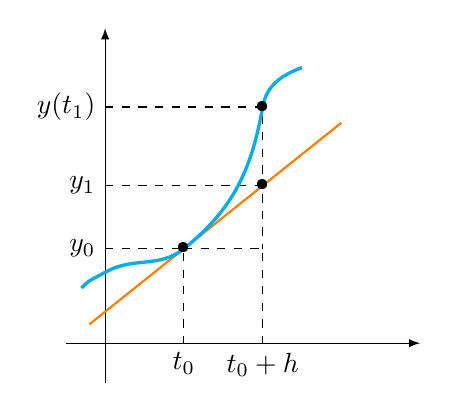
\begin{tikzpicture}[x=1cm,y=1cm]\centering
    \draw[-latex] (-0.5,0)--(4,0); % eixo x
    \draw[-latex] (0,-0.5)--(0,4); % eixo y

    \draw[dashed] (0,1.2) node[left] {$y_0$}--(1,1.2)--(1,0) node[below] {$t_0$}; % y0 -- * -- t0
    \draw[dashed] (1,1.2)--(2,1.2)--(2,0) node[below] {$t_0+h$}; % * -- * -- t_1 = t0+h
    \draw[dashed] (0,2) node[left] {$y_1$}--(2,2)--(2,1.2); % y1 -- * -- t_1 = t0+h
    \draw[dashed] (0,3) node[left] {$y(t_1)$}--(2,3)--(2,2); % y(t1) -- * -- *

    % reta passando pelos pontos (t0, y0) e (t0+h,y1)
    \draw[thick, orange] (-0.2,0.24) -- (3,2.8);

    % a curva
    \draw[very thick, cyan] (-0.3,0.7) 
    to[out=50,in=210] (0,0.9) 
    to[out=30,in=218.66] (1,1.2) 
    to[out=38.66,in=260] (2,3)
    to[out=80,in=200] (2.5,3.5);

    % pontos pretos (bullet)
    \foreach \Point in {(1,1.2),(2,2),(2,3)}{
        \node at \Point {\textbullet};
    }
\end{tikzpicture}
    \caption{Visualização geométrica do método de Euler explícito, onde a curva é a solução exata e a reta é a solução aproximada.}
    \label{fig:euler_explicito_grafico}
\end{figure}

O método de Euler explícito é assim chamado pois fornece explicitamente a sua aproximação em função do instante e do passo anterior, como pode ser visualizado na figura \ref{fig:euler_explicito_grafico}. Uma outra forma de utilizar a primeira derivada é de maneira implícita, no que é chamado \textit{método de Euler implícito}.

\begin{method}[Euler implícito]\label{metodo:euler_implicito}
    Para $h=(b-a)/m$ e $k = 0, 1, ..., m-1$, temos a aproximação:
    \begin{equation*}
        t_{k+1} = t_k + h, \quad
        y_{k+1} = y_k + h f (t_{k+1}, y_{k+1}) = \Phi_h(t_{k+1}, y_{k+1}).
    \end{equation*}
\end{method}

Nesse caso, para avançar a solução no tempo é necessário não apenas aplicar uma fórmula, mas resolver um sistema algébrico de equações geralmente não-lineares no qual $y_{k+1}$ é a incógnita, o que não só exige mais processamento quando utilizado na prática como também pode acumular erros que estão além do método utilizado. Por exemplo, nesses casos é comum utilizar algum método de ponto fixo ou mesmo métodos de Newton ou Quasi-Newton, sendo que nos últimos casos é necessária a estimativa numérica de uma matriz jacobiana $n \times n$ e um certo número de iterações para garantir convergência, o que é custoso e, como todo método numérico, agrega com mais um erro acumulado. Por conta de tudo isso, os métodos numéricos implícitos não foram utilizados nas maiores simulações e não serão tratados neste trabalho. Ainda assim, tais métodos contam com certas vantagens que serão comentadas no decorrer do texto. Mais detalhes dos métodos implícitos e seu uso podem ser encontrados em \cite{Hairer2006-oz}.

Quanto à consistência e à convergência, os métodos propostos são consistentes com 1ª ordem de convergência, pois
\begin{align*}
    e_h(t_{k+1}) 
    &= y(t_{k+1}) - \Phi_h(t_k, \vet y(t_k)) \\
    &= \left(y(t_k) + h \dvet y(t_k) + \dfrac{h^2}{2!} \ddvet y(\xi)\right) - \left( \vet y(t_k) + h f(t_k, \vet y_k) \right) \\
    & = \dfrac{h^2}{2} \ddvet y(\xi),
    \quad
    \xi \in (t_k, t_{k+1}),
\end{align*}
o que pela definição \ref{def:convergencia} implica a ordem 1.

Para exemplificar, considere o problema-modelo \ref{probmodelo:lemniscata} aplicado nos métodos descritos com tamanhos de passo $1/20$, $1/40$, ..., $1/1280$. O resultado pode ser visualizado na tabela \ref{tab:euler_exp_imp_lemniscata}.

\begin{table}[]
    \centering
    \begin{tabular}{c|cc}
        $h$      & Explícito & Implícito   \\
        \hline
        $1/40$   & $0.712071$ & $1.859924$ \\
        $1/80$   & $0.827102$ & $1.283719$ \\
        $1/160$  & $0.904085$ & $1.122329$ \\
        $1/320$  & $0.949289$ & $1.057240$ \\
        $1/640$  & $0.973898$ & $1.027730$ \\
    \end{tabular}
    \caption{Convergência dos métodos de Euler explícito e implícito no problema-modelo \ref{probmodelo:lemniscata}.}
    \label{tab:euler_exp_imp_lemniscata}
\end{table}

Para a aplicação do método de Euler implícito foi utilizado o método de ponto fixo
\begin{equation*}
    \vet y_{k+1}^{[0]} = \vet y_k, \quad \vet y_{k+1}^{[i+1]} = \vet y_k + h f(t_{k+1}, \vet y_{k+1}^{[i]}),
\end{equation*}
para $i=1,...,Q$. Existem diversos critérios para a aplicação deste método \citep[325-335]{Hairer2006-oz}. Porém, como o método não foi de fato utilizado em mais nenhuma outra situação e não foi de nosso interesse neste momento trabalhar com os métodos implícitos no geral, $Q$ foi fixado para $Q=100$ e isso foi mais que suficiente para convergência.


%%%%%%%%%%%%%%%%%%%%%%%%%%%%%%%%%%%%%%%%%%%%%%%%%%%%%%%%%%%%%%%%%
% > METODOS DE RUNGE-KUTTA
%%%%%%%%%%%%%%%%%%%%%%%%%%%%%%%%%%%%%%%%%%%%%%%%%%%%%%%%%%%%%%%%%
\subsection{Métodos de Runge-Kutta}
Uma primeira ideia para obter métodos de ordem mais alta pode ser utilizar séries de Taylor, uma vez que o próprio método de Euler explícito pode ser encontrado via Taylor. O método resultante é como segue.

\begin{method}[Série de Taylor]\label{metodo:taylor}
    Suponha que $f$ do problema \ref{eq:problema_de_cauchy} é de ordem no mínimo $\continuo^q$, e seja $h$ um tamanho de passo fixo. Então
    \begin{equation*}
        \vet \Phi_h(t, \vet y) = y_k + h f(t, \vet y) + \dfrac{h^2}{2!} Df(y,\vet y) + \dfrac{h^3}{3!} D^2 f(t,\vet y) + \hdots + \dfrac{h^q}{q!} D^{q-1} f(t, \vet y),
    \end{equation*}
    onde $D = \derpar{}{t} + f \derpar{}{\vet y}$.
\end{method}

É possível verificar que tal método tem ordem $q$ \citep[42]{alexandre_megiorin_roma_metodos_nodate}. No entanto, tal método traz uma barreira no geral intransponível de maneira analítica para problemas práticos: é preciso encontrar as $q-1$ derivadas de $f$.

Os métodos de Runge-Kutta surgem nesse contexto, a partir da generalização do método de Euler para ordens mais altas, permitindo obter um método de passo único explícito, que concorda com o método \ref{metodo:taylor} para uma dada ordem $q$ e que substitui o cálculo das derivadas de $f$ por médias ponderadas e aplicações de $f$, ou \textit{estágios}, em pontos estratégicos.

\begin{method}[Runge-Kutta de $R$-estágios]\label{metodo:rk_r_estagios}
    Considere o problema \ref{eq:problema_de_cauchy} e tome um tamanho de passo $h$ fixo. Temos
    \begin{equation*}
        \Phi_h(t_k, \vet y_k) = \vet y_k + h \sum_{r=1}^{R} b_r \vet \kappa_r = \vet y_k + h \vet b^T \bm K,
        \quad \bm K = (\kappa_1, ..., \kappa_R)
    \end{equation*}
    onde
    \begin{align*}
        \vet \kappa_r (t,\vet y) &= f\left(t + h c_r, \vet y + h \sum_{j=1}^R a_{rj} \vet \kappa_j \right),
        \quad 1 \leq r \leq R.
    \end{align*}
\end{method}

Os parâmetros $a_{rj}$, $b_r$ e $c_r$ variam para cada método, mas para métodos explícitos sempre satisfazem as relações
\begin{equation}\label{eq:hipoteses_runge_kutta_explicito}
    \begin{aligned}
        \text{(i)} \quad & \sum_{r=1}^{R} b_r = 1, \\
        \text{(ii)} \quad & c_r = \sum_{j=1}^{r-1} a_{rj}, \quad 2 \leq r \leq R.
    \end{aligned}
\end{equation}

A condição (i) é suficiente e necessária para consistência, pois $h \to 0$ leva $\vet \kappa_r (t, \vet y) \to f (t, \vet y)$, então
\begin{equation*}
    \sum_{r=1}^{R} b_r \vet \kappa_r  = f(t,y) \sum_{r=1}^R b_r = f(t,\vet y).
\end{equation*}
Já (ii) garante a concordância com o método de Taylor, conforme \cite[45]{alexandre_megiorin_roma_metodos_nodate}.

Uma notação comum para representar as constantes $a_{rj}$, $b_r$ e $c_r$ é a Tabela de Butcher, dada pela seguinte forma:
\begin{table}
    \centering
    \begin{tabular}{c|c}
         $\vet c$ & $\bm A$\\
         \hline
                  & $\vet b$
    \end{tabular}
    \caption{Tabela de Butcher.}
\end{table}

Observe que o método de Euler explícito (método \ref{metodo:euler_explicito}) é um método de Runge-Kutta de ordem 1 com tabela
\begin{table}
    \centering
    \begin{tabular}{c|ccccc}
         $0$      & \\
         \hline
                  & 1
    \end{tabular}
    \quad
    \begin{tabular}{c|ccccc}
         $1$      & 1  \\
         \hline
                  & 1
    \end{tabular}
    \caption{Tabela de Butcher para os métodos de Euler explícito e implícito, respectivamente.}
\end{table}

Uma grande quantidade de métodos de Runge-Kutta é conhecida, com as mais diferentes ordens. Vale ressaltar também que a ordem de um método de Runge-Kutta é sempre menor ou igual ao número de estágios, ou seja, um método explícito de ordem $p$ tem uma quantidade de estágios $s \geq p$. Mais ainda, se $p \geq 5$, então $s > p$. No geral, parece existir uma tendência de que conforme $p$ aumenta, o valor mínimo de $s$ passa a ser $p + k_p$, para $k_p$ uma constante associada a $p$. Isso, porém, é ainda um problema não resolvido acerca dos métodos de Runge-Kutta \citep[187-196]{Butcher2016-jx}.

Apresentamos a seguir os métodos de ordem 2, 3 e 4, que são os métodos tradicionais mais frequentemente utilizados \citep[46-47]{alexandre_megiorin_roma_metodos_nodate}.

\begin{method}[Runge-Kutta de Segunda Ordem e Dois Estágios (RK22)]\label{metodo:rk22} 
    O método RK22 tem a seguinte Tabela de Butcher:
    \begin{table}[H]
        \centering
        \begin{tabular}{c|cccc}
             $0$      &       &      \\
             $1/2$    & $1/2$  &      \\
             \hline
                      & $0$ & $1$
        \end{tabular}
        \caption{Tabela de Butcher para o método RK22.}
    \end{table}
\end{method}

\begin{method}[Runge-Kutta de Terceira Ordem e Três Estágios (RK33)]\label{metodo:rk33} 
    O método RK33 tem a seguinte Tabela de Butcher:
    \begin{table}[H]
        \centering
        \begin{tabular}{c|cccc}
             $0$      &       &       &     \\
             $1/2$    & $1/2$ &       &     \\
             $1$      & $-1$   & $2$  &     \\
             \hline
                      & $1/6$ & $4/6$ & $1/6$
        \end{tabular}
        \caption{Tabela de Butcher para o método RK33.}
    \end{table}
\end{method}

\begin{method}[Runge-Kutta de Quarta Ordem e Quatro Estágios (RK44)]\label{metodo:rk44} 
    O método RK44 tem a seguinte Tabela de Butcher:
    \begin{table}[H]
        \centering
        \begin{tabular}{c|ccccc}
             $0$      &       &       &       &\\
             $1/2$    & $1/2$ &       &       &\\
             $1/2$    & $0$   & $1/2$ &       &\\
             $1$      & $0$   & $0$   & $1$   & \\
             \hline
                      & $1/6$ & $1/3$ & $1/3$ & $1/6$
        \end{tabular}
        \caption{Tabela de Butcher para o método RK44.}
    \end{table}
\end{method}

O mesmo método para depuração da ordem dos métodos (ver (\ref{eq:aproximacao_ordem})) pode ser aplicado para os métodos de Runge-Kutta no problema-modelo \ref{probmodelo:lemniscata}. O resultado consta na tabela \ref{tab:rk_lemniscata}.

\begin{table}[]
    \centering
    \begin{tabular}{c|ccc}
        $h$     & RK22 & RK33 & RK44 \\
        \hline
        $1/40$  & $1.989241$ & $2.936490$ & $4.041771$ \\
        $1/80$  & $2.003212$ & $2.965188$ & $4.025951$ \\
        $1/160$ & $2.003873$ & $2.981701$ & $4.014280$ \\
        $1/320$ & $2.002516$ & $2.990612$ & $4.008214$ \\
        $1/640$ & $2.001404$ & $2.995243$ & $3.992159$ \\
    \end{tabular}
    \caption{Convergência dos métodos RK22, RK33 e RK44 no problema-modelo \ref{probmodelo:lemniscata}}
    \label{tab:rk_lemniscata}
\end{table}


%%%%%%%%%%%%%%%%%%%%%%%%%%%%%%%%%%%%%%%%%%%%%%%%%%%%%%%%%%%%%%%%%
% > ESTABILIDADE DOS METODOS TRADICIONAIS
%%%%%%%%%%%%%%%%%%%%%%%%%%%%%%%%%%%%%%%%%%%%%%%%%%%%%%%%%%%%%%%%%
\subsection{Estabilidade dos integradores tradicionais}
Outra questão importante a se analisar sobre integradores numéricos é como se comportam em intervalos ilimitados, não apenas em intervalos limitados como feito até então. Para isso, é utilizado como problema modelo o problema de valor inicial mais simples possível:
\begin{equation}\label{eq:edo_problema_linear}
    \dvet y(t) = \bm M \vet y(t), \quad \vet y(t_0) = \vet y_0,
\end{equation}
sendo $\bm M$ uma matriz constante. O método de Euler explícito aplicado com um tamanho de passo $h$ assume a seguinte forma para o instante $t_k = t_0 + k h$:
\begin{equation}\label{eq:edo_linear_aproximacao}
    \vet y_k = (\bm I + h \bm M) \vet y_{k-1}
    \quad
    \therefore
    \quad
    \vet y_k = (\bm I + h \bm M)^k \vet y_0.   
\end{equation}
Além disso, da teoria de equações diferenciais, sabemos que a solução exata do problema (\ref{eq:edo_problema_linear}) é
\begin{equation}\label{eq:edo_linear_solucao}
    \vet y(t_k) = \exp{(k h \bm M)} \vet y_0.
\end{equation}

Considere uma mudança de base tal que $\vet y(t) = \bm A \vet z(t)$ e $\vet y_k = \bm A \vet z_k$, sendo $\bm A$ uma matriz constante e não singular. Temos então o problema nas novas coordenadas:
\begin{equation}
    \dvet z (t) = \bm A^{-1} \bm M \bm A \vet z(t) = \bm B \vet z(t),
    \quad
    \vet z(t_0) = \vet z_0,
\end{equation}
com solução exata
\begin{equation}
    \vet z(t_k) = \exp{(k h \bm B)} \vet z_0
\end{equation}
e solução aproximada
\begin{equation}
    \vet z_k = (\bm I + h \bm B)^k \vet z_0.
\end{equation}
Se a transformação escolhida é tal que $\bm B$ é a forma canônica de Jordan de $\bm M$, então para cada autovalor $\lambda$ tem-se uma equação diferencial da forma
\begin{equation}
    \dvet y(t) = \lambda \vet y(t),
\end{equation}
chamada \textbf{problema modelo} se $\RePart{\lambda} < 0$, com solução
\begin{equation}
    \vet y(t_k) = \exp{(k h \lambda}) \vet y_0.
\end{equation}
Assim, para o método de Euler explícito ser adequado é necessário que $(1+ h \lambda)^k$ seja uma aproximação aceitável para $\exp{(k h \lambda)}$, ou que no mínimo $(1+h \lambda)^k$ tenha comportamento limitado para $k \to \infty$ quando $\exp{(k h \lambda)}$ for limitado. Isso ocorre se e somente se $|1 + h \lambda| \leq 1$. Tomando $z = h \lambda$, a região complexa $|1+z| \leq 1$ é chamada de \textbf{região estável} para o método de Euler explícito, conforme figura \ref{fig:regiao_estabilidade_euler_explicito}.

\begin{figure}
    \centering
    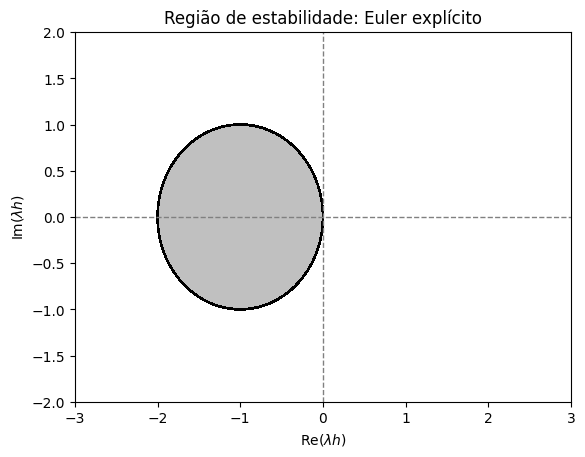
\includegraphics[width=0.5\linewidth]{tcc//img/regiao_estabilidade_euler.png}
    \caption{Região de estabilidade para o método de Euler explícito.}
    \label{fig:regiao_estabilidade_euler_explicito}
\end{figure}

\begin{definition}[Estabilidade de métodos numéricos]
    O problema de valor inicial
    \begin{equation*}
        \dot y(t) = \lambda y(t),
        \quad
        y(t_0) = y_0,
        \quad \RePart{\lambda} < 0
    \end{equation*}
    é chamado de \textbf{problema modelo}. Considere um método de passo único que aplicado ao problema modelo fornece a expressão
    \begin{equation*}
        y_{k+1} = \phi (\lambda h) y_k.
    \end{equation*}
    O conjunto $\Omega = \{\eta \in \mathbb{C} : |\phi(\eta)| < 1 \}$ é denominado \textbf{região de estabilidade absoluta} para $h>0$ fixado, $\phi(\lambda h)$ é chamado \textbf{fator de amplificação} e o intervalo $I_e = \Omega \cap \R$ é o \textbf{intervalo de estabilidade absoluta} do método. Um método \textbf{absolutamente estável} é também chamado de \textbf{A-estável}.
\end{definition}

Observando a região de estabilidade do método de Euler explícito, é fácil concluir que o método não é A-estável, uma vez que $|1+h \lambda| \leq 1$ somente se $h \leq - \RePart{\lambda} / |\lambda|$. Dizemos então que trata-se de um método \textbf{condicionalmente estável}.

Por outro lado, o método de Euler implícito (método \ref{metodo:euler_implicito}) tem uma comportamento diferente. Aplicando o mesmo processo anterior, obtemos a expressão
\begin{equation}
    \vet y_k = (1 - z)^{-1} \vet y_{k-1},
\end{equation}
e então sua região estável é $|1-z| \geq 1$, como na figura \ref{fig:regiao_estabilidade_euler_implicito}. Nesse caso, $\phi (\lambda h) = (1 - \lambda h)^{-1}$, então para qualquer $h > 0$ temos que $|\phi(\lambda h)| < 1$.

\begin{figure}
    \centering
    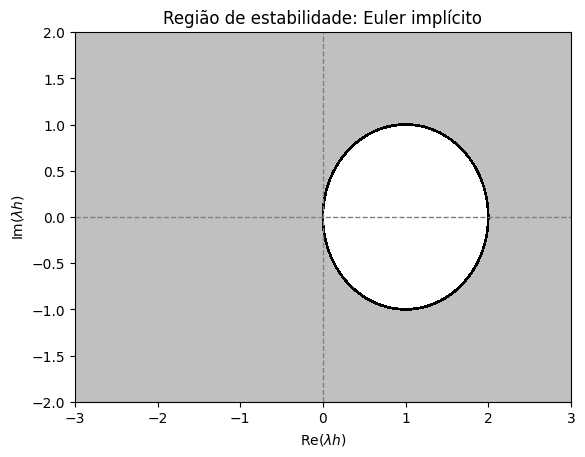
\includegraphics[width=0.5\linewidth]{tcc/img/regiao_estabilidade_euler_implicito.png}
    \caption{Região de estabilidade do método de Euler implícito}
    \label{fig:regiao_estabilidade_euler_implicito}
\end{figure}

É possível generalizar essa ideia para os métodos de Runge-Kutta. Tomando um método de ordem $s$ com tabela
\begin{table}
    \centering
    \begin{tabular}{c|c}
        $\vet c$ &  $\bm A$ \\
        \hline & $\vet b^T$
    \end{tabular}
\end{table}\\
temos para o problema modelo:
\begin{equation}
    \bm K = (\bm I - h \lambda \bm A)^{-1} \lambda \bm 1 y_0
    = (\bm I - z \bm A)^{-1} \lambda \bm 1 y_0,
\end{equation}
então
\begin{equation}\label{eq:ampliacao_rk_geral}
    y_1 
    = y_0 + h \vet b^T \bm K
    = [1 + z \vet b^T (\bm I - z \bm A)^{-1} \bm 1] y_0
    = R(z) y_0,
\end{equation}
sendo $R(\vet z)$ o fator de ampliação do método. Para o caso de métodos explícitos, a matriz $\bm A$ é triangular com diagonal nula, e portanto nilpotente com algum grau $k$. Através de uma expansão algébrica pode-se concluir que
\begin{equation}\label{eq:inversa_nilpotentes}
    (\bm I - z \bm A) = \bm I + \sum_{j=1}^{k-1} z^j \bm A^k.
\end{equation}
Substituindo (\ref{eq:inversa_nilpotentes}) em (\ref{eq:ampliacao_rk_geral}),
\begin{align*}
    R(z) 
    &= 1 + z \vet b^T (\bm I + \sum_{j=1}^{k-1} z^j \bm A^j)\bm 1 \\
    &= 1 + z \vet b^T \bm I \bm 1 + \vet b^T \sum_{j=1}^{k-1} z^{j+1} \bm A^j \bm 1.
\end{align*}
A partir de (\ref{eq:hipoteses_runge_kutta_explicito}), temos por (i) que $\vet b^T \bm I \bm 1 = \sum_{j=1}^s b_j = 1$. Temos então que
\begin{equation}
    R(z) = 1 + z + \sum_{j=1}^{k-1} z^{j+1} \bm A^j \bm 1.
\end{equation}
No caso dos métodos explícitos em que $p=s$, temos os seguintes fatores:
\begin{equation}
    R (z) = \begin{cases}
    1 + z, & p = 1, \\
    1 + z + \frac{1}{2} z^2, & p = 2, \\
    1 + z + \frac{1}{2} z^2 + \frac{1}{6} z^3, & p = 3, \\
    1 + z + \frac{1}{2} z^2 + \frac{1}{6} z^3 + \frac{1}{24} z^4, & p = 4.
    \end{cases}
\end{equation}
A região de estabilidade absoluta desses métodos pode ser vista na figura \ref{fig:regiao_estabilidade_rk_explicitos}, sendo o interior de cada curva fechada.

\begin{figure}
    \centering
    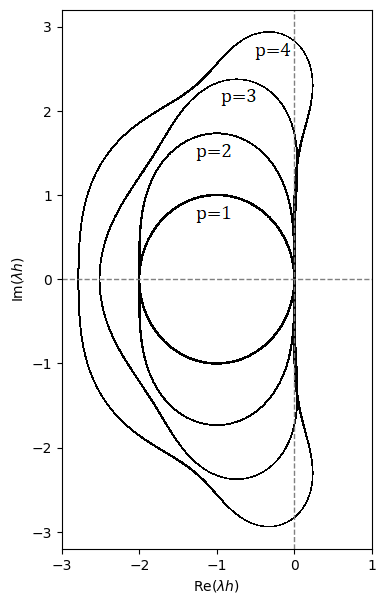
\includegraphics[width=0.35\linewidth]{tcc//img/regiao_estabilidade_rk.png}
    \caption{Região de estabilidade dos métodos de Runge-Kutta de ordens e estágios $p = 1, 2, 3$ e $4$.}
    \label{fig:regiao_estabilidade_rk_explicitos}
\end{figure}

Uma vez que as regiões de estabilidade são fechadas pois o fator é polinomial, os métodos de Runge-Kutta explícitos não são A-estáveis. Porém, da mesma forma que no caso dos métodos de Euler explícito e implícito, é possível obter A-estabilidade utilizando métodos implícitos. 
\begin{table}[H]
    \centering

    \begin{tabular}{c|cc}
        $\frac{1}{2} - \frac{\sqrt 3}{6}$ & $1/4$ & $\frac{1}{4} - \frac{\sqrt 3}{6}$ \\
        $\frac{1}{2} + \frac{\sqrt 3}{6}$ & $\frac{1}{4} + \frac{\sqrt 3}{6}$ & $1/4$ \\
        \hline & $1/2$ & $1/2$
    \end{tabular}
    
    \caption{Método de Runge-Kutta implícito de quarta ordem e dois estágios. \citep[99]{Butcher2016-jx}}.
    \label{tab:exemplo_metodo_runge_kutta_implicito}
\end{table}

Por exemplo, considere o método de quarta ordem da tabela \ref{tab:exemplo_metodo_runge_kutta_implicito}. Seu fator de amplificação é
\begin{equation*}
    R(z) = \dfrac{1 + \frac{z}{2} + \frac{z^2}{12}}{1 - \frac{z}{2} + \frac{z^2}{12}}.
\end{equation*}
Observe que $|R(z)| \leq 1$ somente se $\RePart{z} \leq 0$, e uma vez que $z = \lambda h$ com $\RePart{\lambda} < 0$, qualquer valor de $h$ garante estabilidade para o método, sendo então A-estável.

Apesar da maior facilidade para obter métodos implícitos de altas ordens e estáveis, a necessidade de utilizar métodos iterativos para resolver o sistema de equações pode não compensar computacionalmente tais ganhos qualitativos. Ainda assim, os métodos de Runge-Kutta implícitos são utilizados em diversas aplicações, inclusive porque todas as versões simpléticas dos métodos RK são necessariamente implícitas (veja o Teorema \ref{teorema:rk_simpletico}).

De toda forma, a A-estabilidade, por definição, se aplica para problemas lineares, o que não é o caso da grande maioria de aplicações práticas dos integradores numéricos. No entanto, muitos sistemas podem ser aproximados localmente por sua linearização, sendo então possível aplicar os resultados de estabilidade para obter tamanhos de passo adequados.

No problema de N-corpos, utilizar o método de Euler implícito não apresentou nenhuma vantagem. No entanto, ainda é possível observar algumas anomalias esperadas para cada método simulando, por exemplo, o problema-modelo \ref{probmodelo:lemniscata}. Na figura \ref{fig:lemniscata_euler_exp_imp_distancia} é possível observar a diferença na divergência entre os dois métodos quando comparados a um método simplético de alta ordem. Enquanto o método de Euler explícito apresenta um afastamento de órbita mais prolongado, o método de Euler implícito apresenta afastamentos mais breves.

\begin{figure}
    \centering
    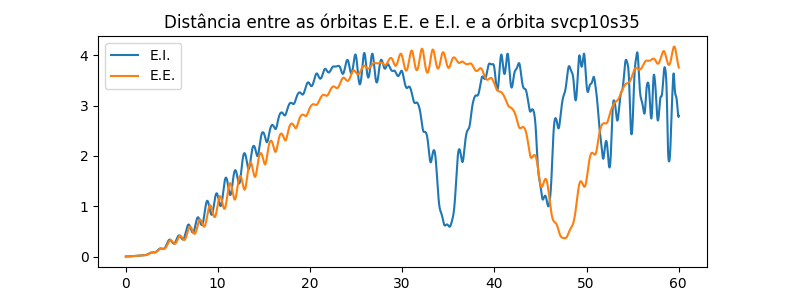
\includegraphics[width=0.75\linewidth]{tcc//img/lemniscata_euler_exp_imp_svcp10s35.png}
    \caption{Distância no espaço de fases entre as soluções numéricas do problema-modelo \ref{probmodelo:lemniscata} com métodos de Euler explícito e implícito e o método svcp10s35 com $h=10^{-3}$ no intervalo $[0,60]$.}
    \label{fig:lemniscata_euler_exp_imp_distancia}
\end{figure}

Um motivo para isso pode ser observado na figura \ref{fig:lemniscata_euler_exp_imp}. Uma vez que $E_0 - E$ decresce no método de Euler explícito, a energia total está aumentando, o que significa que a energia cinética está aumentando (ou que a potencial está diminuindo). Isso leva a um relaxamento do período e com aproximações mais violentas, e portanto ao menos uma partícula deve ser ejetada do sistema em sua evolução.

Já no caso implícito, $E_0-E$ cresce, logo a energia total está diminuindo, então a energia potencial está aumentando (ou a energia cinética está diminuindo). Isso implica no encolhimento do período, e como o PNCG pode conter colisões o sistema fica numericamente instável.

Na prática, o método de Euler explícito ``erra para mais'', expandindo a trajetória, enquanto o método de Euler implícito ``erra para menos'', contraindo a trajetória.

\begin{figure}
        \centering
        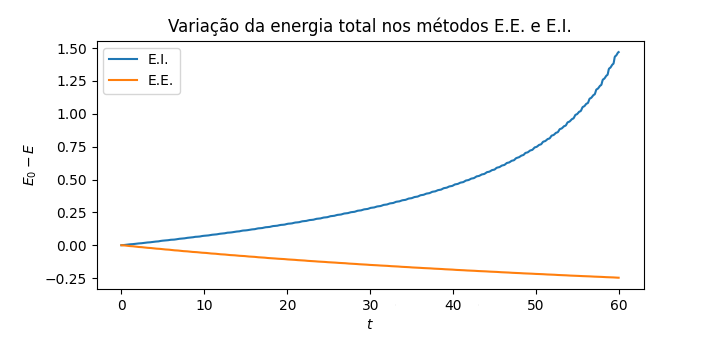
\includegraphics[width=0.7\linewidth]{tcc//img/lemniscata_euler_exp_imp.png}
        \caption{Variação (com sinal) da energia total em simulações do problema-modelo \ref{probmodelo:lemniscata} via métodos de Euler explícito e implícito e com $h=10^{-3}$ no intervalo $[0,60]$.}
        \label{fig:lemniscata_euler_exp_imp}
\end{figure}

%%%%%%%%%%%%%%%%%%%%%%%%%%%%%%%%%%%%%%%
%%% METODOS SIMPLÉTICOS
%   Ideia inicial dos métodos;
%   Estabilidade e afins;
%   Exemplos de métodos:
%       Euler Simplético (1a Ordem);
%       Velocity-Verlet (2a Ordem);
%       Ruth3 e Ruth4 (3a e 4a Ordem);
%       RKN551 e RKN671 (5a e 6a Ordem);
%       SVCP8S15 e SVCP10S35 (8a e 10a Ordem).
%   Comparacao numerica com os métodos tradicionais;
%%%%%%%%%%%%%%%%%%%%%%%%%%%%%%%%%%%%%%%
% IDEIA INICIAL:
%   Ideia inicial dos métodos;
%   Propriedades
%   Exemplos de métodos:
%       Euler Simplético (1a Ordem);
%       Velocity-Verlet (2a Ordem);
%       Ruth3 e Ruth4 (3a e 4a Ordem);
%       RKN551 e RKN671 (5a e 6a Ordem);
%       SVCP8S15 e SVCP10S35 (8a e 10a Ordem).
%   Comparacao numerica com os métodos tradicionais;

\section{Integradores simpléticos}\label{secao:integradores_simpleticos}
Como apresentado brevemente na introdução deste capítulo, os métodos simpléticos se baseiam na estrutura do espaço de fases, e não apenas na função que está sendo integrada. Nesse sentido, tais métodos são construídos de modo a preservarem a estrutura simplética dos problemas hamiltonianos, conservando o volume da solução e consequentemente conservando as integrais primeiras também.

Essas diferenças na forma e objetivo de construir os integradores entre os métodos tradicionais e os simpléticos têm implicações importantes sobre os resultados. Os métodos tradicionais são construídos tendo-se em vista uma estabilidade assintótica do sistema, imbuindo dissipações na solução numérica que distorcem as trajetórias de sistemas hamiltonianos, ainda que sejam aplicados integradores tradicionais de alta ordem, como exemplificado ao final da seção anterior. Isso não ocorre com integradores simpléticos, como apresentamos a seguir.

Para esta seção, no lugar de considerar um problema de Cauchy qualquer, tomaremos aqueles que podem ser escritos através das equações de Hamilton:
\begin{equation}\label{eq:pvi_hamilton}
    \dvet z(t) = \bm \Omega \nabla_{\vet z} H(\vet z),
    \quad
    \vet z(0) = \vet z_0,
    \quad
    \vet z(t) = (\vet q(t), \vet p(t)),
    \quad
    \bm \Omega = \begin{bmatrix}
        \bm 0 & \bm I \\ - \bm I & \bm 0
    \end{bmatrix}.
\end{equation}

Como já apresentado no capítulo \ref{capitulo:revisao_mecanica}, o fluxo do problema (\ref{eq:pvi_hamilton}) é \textit{simplético}, ou seja, conserva o volume no espaço de fases. Em particular, isso significa que conserva também as integrais primeiras do sistema. A proposta dos \textit{integradores simpléticos} é fornecer uma aplicação simplética $\vet \Phi_h$ tal que
\begin{equation*}
    \vet z_1 = \vet \Phi_h(\vet z_0).
\end{equation*}
Ademais, conforme o teorema \ref{teorema:simpleticidade_matricial}, um critério para $\vet \Phi_h$ ser simplética é ser tal que
\begin{equation*}
    D \Phi_h \bm \Omega D \Phi_h^T = \bm \Omega.
\end{equation*}


\subsection{Obtenção de métodos via separação}
Quando a função hamiltoniana é separável, ou seja, $H(\vet q, \vet p) = T(\vet p) + V(\vet q)$, é possível obter métodos explícitos a partir do que segue. Tomando como hamiltoniano primeiramente apenas $T$ e em seguida apenas $V$, temos os dois problemas de valor inicial respectivos:
\begin{equation}
    \begin{cases}
        \dvet q = \nabla_{\vet p} T(\vet p) = \dfrac{1}{m} \vet p, \\
        \dvet p = \vet 0,
    \end{cases},
    \quad
    \begin{cases}
        \dvet q = \vet 0, \\
        \dvet p = - \nabla_{\vet q} V(\vet q) = F(\vet q).
    \end{cases}   
\end{equation}
Em ambos os casos, podemos obter o fluxo de maneira explícita, uma vez que uma das coordenadas está constante:
\begin{equation}
    \vet \Phi_{\tau, T} (\vet z) = \begin{bmatrix}
        \vet q + \tau \vet p/m \\ \vet p
    \end{bmatrix},
    \quad
    \vet \Phi_{\tau, V} (\vet z) = \begin{bmatrix}
        \vet q \\ \vet p + \tau \vet F(\vet q)
    \end{bmatrix}.
\end{equation}
Se tomamos a aplicação composta $\vet \Phi_{\tau} := \vet \Phi_{\tau, T} \circ \vet \Phi_{\tau, V}$, obtemos um primeiro método com semblante familiar.

\begin{method}[Euler Simplético (ou semi-implícito)]\label{metodo:euler_simpletico}
    Para um tamanho de passo $h$ fixo em um intervalo discretizado para um problema de valor inicial hamiltoniano separável, temos a aproximação:
    \begin{equation}
        \vet q_{k+1} = \vet q_k + h \dfrac{\vet p_{k+1}}{m},
        \quad
        \vet p_{k+1} = \vet p_k + h \vet F(\vet q_k).
    \end{equation}
\end{method}

Da mesma forma que os métodos de Euler explícito e implícito (métodos \ref{metodo:euler_explicito} e \ref{metodo:euler_implicito}, respectivamente), o método de Euler simplético tem ordem 1 \citep[189]{Hairer2006-oz}. No entanto, trata-se de um método simplético, pois vale o critério matricial (Teorema \ref{teorema:simpleticidade_matricial}):
\begin{equation*}
    D \vet \Phi_h = \begin{bmatrix}
        1 + \dfrac{h^2}{m} \nabla_{\vet q} \vet F(\vet q) & \dfrac{h}{m} \\
        h \nabla_{\vet q} \vet F(\vet q) & 1
    \end{bmatrix}
    \quad
    \Longrightarrow
    \quad
    D \vet \Phi_h \bm \Omega D \vet \Phi_h^T = \begin{bmatrix}
        \vet 0 & \bm I \\ - \bm I & \vet 0
    \end{bmatrix}
    = \bm \Omega.
\end{equation*}

A diferença entre os métodos pode ser observada aplicando-os no problema-modelo \ref{probmodelo:lemniscata}, como na figura \ref{fig:var_energia_rk22_rk33_rk44_es}. Veja que embora todos os métodos de Runge-Kutta (com ordem maior que 1) comecem com uma variação menor de energia que o método de Euler simplético (com ordem 1), a variação do segundo é relativamente preservada, enquanto que a dos métodos RK escalona. No caso do RK44, embora a precisão seja mantida por mais tempo para $h=0.05$, um tamanho de passo $h=0.15$ permite visualizar melhor o erro na energia escalonando.

\begin{figure}
    \centering
    \begin{subfigure}{.5\textwidth}
      \centering
      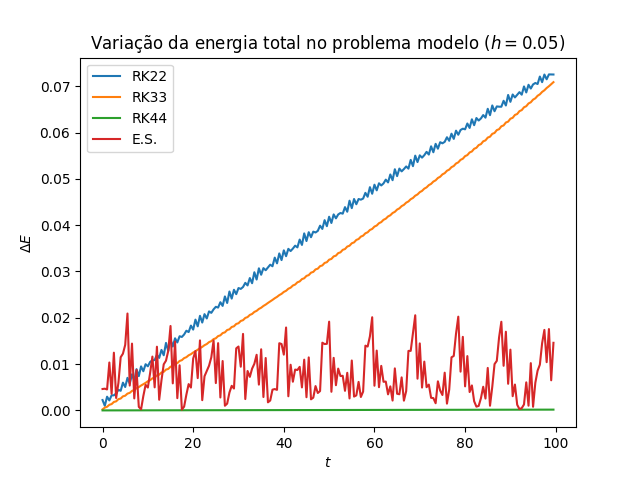
\includegraphics[width=\linewidth]{tcc/img/var_energia_rk22_rk33_rk44_es.png}
      \caption{Intervalo $[0,100]$ e $h=0.05$.}
      \label{fig:var_energia_rk22_rk33_rk44_es_a}
    \end{subfigure}%
    \begin{subfigure}{.5\textwidth}
      \centering
      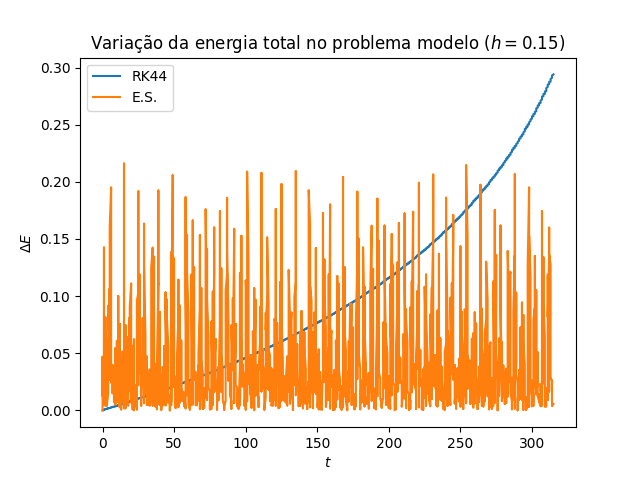
\includegraphics[width=\linewidth]{tcc/img/var_energia_rk44_es.png}
      \caption{Intervalo $[0,300]$ e $h=0.15$.}
      \label{fig:var_energia_rk22_rk33_rk44_es_b}
    \end{subfigure}
    \caption{Variação da energia total na simulação do problema-modelo \ref{probmodelo:lemniscata} com os métodos RK22, RK33, RK44 e Euler Simplético (E.S.)}
    \label{fig:var_energia_rk22_rk33_rk44_es}
\end{figure}

A ideia de composição também pode ser aplicada para obter métodos com ordem mais alta. Tomando constantes de peso (isto é, que somam 1) $c_1, ..., c_s$ e $d_1, ..., d_s$, tomamos a composição
\begin{equation*}
    \vet \Phi_h = \vet \Phi_{d_s h, V} \circ \vet \Phi_{c_s h, T} \circ \hdots \circ \vet \Phi_{d_1 h, V} \circ \vet \Phi_{c_1 h, T}.
\end{equation*}
Conforme \cite[145-146]{Leimkuhler2005}, métodos $\vet \Phi_h$ com esta forma são consistentes e, além disso, se os coeficientes são simétricos ($c_i = c_{s+1-i}$ e $d_i = d_{s+1-i}$), então o método tem no mínimo ordem 2.

\begin{method}[Velocity-Verlet]\label{metodo:velocity-verlet}
    Tomando os coeficientes $d_1=d_2=1/2$, $c_1 = 0$ e $c_2=1$, obtemos um método consistente, simétrico, explícito, simplético e de segunda ordem dado por
    \begin{align*}
        \vet q_{k+1} &= \vet q_k + h \dfrac{\vet p_k}{m} + \dfrac{h^2}{2 m} \vet F(\vet q_k), 
        \\
        \vet p_{k+1} &= \vet p_k + \dfrac{h}{2} (\vet F(\vet q) + \vet F(\vet q_{k+1})).
    \end{align*}
\end{method}

\begin{theorem}
    O método Velocity-Verlet é simplético.
\end{theorem}
\begin{Proof}
    Seja $\vet \Phi_h (\vet q, \vet p) = (\vet Q (\vet q, \vet p), \vet P(\vet q, \vet p))$. Então:
    \begin{align*}
        \derpar{\vet Q}{\vet q} &= 1 + \dfrac{1}{2} \dfrac{h^2}{m} \derpar{\vet F}{\vet q}, 
        &\quad
        \derpar{\vet Q}{\vet p} &= \dfrac{h}{m}, 
        \\
        \derpar{\vet P}{\vet q} &= \dfrac{h}{2} \derpar{\vet F}{\vet q} \left(1 + \derpar{\vet Q}{\vet q}\right),
        &\quad
        \derpar{\vet P}{\vet p} &= \derpar{\vet Q}{\vet q}.
    \end{align*}
    Nesse caso, a condição do teorema \ref{teorema:simpleticidade_matricial} é facilmente verificada:
    \begin{equation*}
        \derpar{\vet Q}{\vet q} \derpar{\vet P}{\vet p} - \derpar{\vet Q}{\vet p} \derpar{\vet P}{\vet q} 
        = \left(\derpar{\vet Q}{\vet q}\right)^2 - \left(\derpar{\vet Q}{\vet q} - 1\right) \left(1 + \derpar{\vet Q}{\vet q}\right) = 1.
    \end{equation*}
\end{Proof}

Outros dois métodos de ordens 3 e 4 foram propostos, respectivamente, por \cite{Ruth1983} e por \cite{Forest1990}.

\begin{method}[Ruth 3]\label{metodo:ruth3}
    Um método simplético de 3ª ordem é obtido através dos coeficientes
    \begin{align*}
        c_1 = 1,    & \quad & c_2 = -2/3, & \quad & c_3 = 2/3, \\
        d_1 = -1/24 & \quad & d_2 = 3/4,  & \quad & d_3 = 7/24.
    \end{align*}
\end{method}

\begin{method}[Ruth 4]\label{metodo:ruth4}
    Um método simplético de 4ª ordem é obtido através dos coeficientes
    \begin{align*}
        c_1 = c_4 = \dfrac{1}{2(2-2^{1/3})}, & \quad & c_2 = c_3 = \dfrac{1-2^{1/3}}{2(2-2^{1/3})}, \\
        d_1 = d_3 = \dfrac{1}{2-2^{1/3}}, & \quad & d_2 = - \dfrac{2^{1/3}}{2-2^{1/3}}, \quad d_4 = 0.
    \end{align*}
\end{method}


\subsection{Métodos via composição de integradores de segunda ordem}
Seguindo nessa linha, \cite{Yoshida1990} observa que uma forma eficiente de obter métodos de alta ordem para problemas com funções hamiltonianas separáveis é através da composição de métodos simétricos de segunda ordem. A facilidade vem dos termos ímpares da expansão de Taylor se anularem, o que simplifica as condições de ordem do método, e procurar por métodos de ordem par é conveniente uma vez que os métodos simétricos sempre têm ordem par e são reversíveis no tempo \citep[147]{Leimkuhler2005}. Vale ressaltar que a composição de simplectomorfismos é também simplectomorfa, o que significa que compôr métodos de Verlet, por exemplo, com uma boa escolha de pesos, fornece integradores simpléticos, simétricos, consistentes e de alta ordem. Nesse caso, as aplicações compostas $\vet \Psi_h$ têm a forma
\begin{equation*}
    \vet \Psi_h = \vet \Phi_{\gamma_s h} \circ \hdots \circ \vet \Phi_{\gamma_2 h} \circ \Phi_{\gamma_1 h},
\end{equation*}
onde $\vet \Phi_{\gamma_i h}$ é o método de Verlet (\ref{metodo:velocity-verlet}) com tamanho de passo $\gamma_i h$, para $i=1,2,...,s$. Dois métodos deste tipo foram implementados no programa final, com ordens 8 e 10.

\begin{method}[svcp8s15]\label{metodo:svcp8s15}\citep[157]{Hairer2006-oz}
    Um método Stormer-Verlet Composto de 8ª ordem e 15 estágios (svc8s15) é obtido através dos coeficientes:
    \begin{center}
        \begin{tabular}{ccccr}        
        $\gamma_1$ &$=$& $\gamma_{15}$ &$=$& $0.74167036435061295344822780$ \\
        $\gamma_2$ &$=$& $\gamma_{14}$ &$=$& $-0.40910082580003159399730010$ \\
        $\gamma_3$ &$=$& $\gamma_{13}$ &$=$& $0.19075471029623837995387626$ \\
        $\gamma_4$ &$=$& $\gamma_{12}$ &$=$& $-0.57386247111608226665638773$ \\
        $\gamma_5$ &$=$& $\gamma_{11}$ &$=$& $0.29906418130365592384446354$ \\
        $\gamma_6$ &$=$& $\gamma_{10}$ &$=$& $0.33462491824529818378495798$ \\
        $\gamma_7$ &$=$& $\gamma_{9}$  &$=$& $0.31529309239676659663205666$ \\
                   &   & $\gamma_{8}$  &$=$& $-0.79688793935291635401978884$ \\
        \end{tabular}
    \end{center}
\end{method}

\begin{method}[svcp10s35]\label{metodo:svcp10s35}\citep[158]{Hairer2006-oz}
    Um método Stormer-Verlet Composto de 10ª ordem e 35 estágios (svc8s15) é obtido através dos coeficientes:
    \begin{center}
        \begin{tabular}{ccccr}        
        $\gamma_1$  &$=$& $\gamma_{35}$ &$=$& $ 0.07879572252168641926390768$ \\
        $\gamma_2$  &$=$& $\gamma_{34}$ &$=$& $ 0.31309610341510852776481247$ \\
        $\gamma_3$  &$=$& $\gamma_{33}$ &$=$& $ 0.02791838323507806610952027$ \\
        $\gamma_4$  &$=$& $\gamma_{32}$ &$=$& $-0.22959284159390709415121340$ \\
        $\gamma_5$  &$=$& $\gamma_{31}$ &$=$& $ 0.13096206107716486317465686$ \\
        $\gamma_6$  &$=$& $\gamma_{30}$ &$=$& $-0.26973340565451071434460973$ \\
        $\gamma_7$  &$=$& $\gamma_{29}$ &$=$& $ 0.07497334315589143566613711$ \\
        $\gamma_8$  &$=$& $\gamma_{28}$ &$=$& $ 0.11199342399981020488957508$ \\
        $\gamma_9$  &$=$& $\gamma_{27}$ &$=$& $ 0.36613344954622675119314812$ \\
        $\gamma_{10}$ &$=$& $\gamma_{26}$ &$=$& $-0.39910563013603589787862981$ \\
        $\gamma_{11}$ &$=$& $\gamma_{25}$ &$=$& $ 0.10308739852747107731580277$ \\
        $\gamma_{12}$ &$=$& $\gamma_{24}$ &$=$& $ 0.41143087395589023782070412$ \\
        $\gamma_{13}$ &$=$& $\gamma_{23}$ &$=$& $-0.00486636058313526176219566$ \\
        $\gamma_{14}$ &$=$& $\gamma_{22}$ &$=$& $-0.39203335370863990644808194$ \\
        $\gamma_{15}$ &$=$& $\gamma_{21}$ &$=$& $ 0.05194250296244964703718290$ \\
        $\gamma_{16}$ &$=$& $\gamma_{20}$ &$=$& $ 0.05066509075992449633587434$ \\
        $\gamma_{17}$ &$=$& $\gamma_{19}$ &$=$& $ 0.04967437063972987905456880$ \\
                    &   & $\gamma_{18}$ &$=$& $ 0.04931773575959453791768001$ \\
        \end{tabular}
    \end{center}
\end{method}

Apesar da relativa facilidade de obter métodos simpléticos através de composição de métodos de primeira e de segunda ordem, é fácil ver pelos métodos \ref{metodo:svcp8s15} e \ref{metodo:svcp10s35} que é necessária uma quantidade de estágios muito maior do que a ordem do método, o que torna a usabilidade dos métodos cada vez mais desafiadora. Porém, existem muitos outros métodos simpléticos e que não são baseados em composição. Dois tipos bastante comuns são os métodos de Runge-Kutta Simpléticos e os métodos de Runge-Kutta-Nyström.

\subsection{Métodos de Runge-Kutta Simpléticos e de Runge-Kutta-Nyström}
Para obter um método de Runge-Kutta simplético basta adicionar uma restrição (além das já apresentadas anteriormente) sobre o método \ref{metodo:rk_r_estagios}.

\begin{theorem}\label{teorema:rk_simpletico}
    Se os coeficientes de um método de Runge-Kutta de $R$ estágios são tais que
    \begin{equation*}
        b_i a_{ij} + b_j a_{ji} - b_i b_j = 0, \quad i, j = 1, ..., R, 
    \end{equation*}
    então trata-se de um método simplético.
\end{theorem}

A demonstração do teorema pode ser encontrada em \cite[152-154]{Leimkuhler2005}. O importante neste momento é que decorre do teorema que para $i=j$ temos
\begin{equation*}
    2 a_{ii} = b_i, \quad \forall i = 1, 2, ..., R.
\end{equation*}
Uma vez que o vetor $\vet b$ não é nulo, isso significa que a matriz de coeficientes $\bm A$ tem diagonal não-nula, e portanto não é possível obter um integrador de Runge-Kutta simplético que seja explícito. Tendo em vista as já mencionadas dificuldades de se trabalhar computacionalmente com métodos implícitos, nenhum método de Runge-Kutta simplético foi testado neste trabalho.

Já os métodos de Runge-Kutta-Nyström (RKN) são voltados especificamente para problemas de valor inicial do tipo
\begin{equation*}
    \ddvet x = g(t, \vet x, \dvet x),
\end{equation*}
então são aplicáveis para grande parte dos problemas de mecânica hamiltoniana, como o PNCG. O método geral é dado pelo que segue.

\begin{method}[Runge-Kutta-Nyström de $s$ estágios]\citep[41]{Hairer2006-oz}
    Um método RKN de $s$ estágios para um sistema hamiltoniano separável em $T$ e $V$ é dado por
    \begin{align*}
        \vet y_i & = \vet q_k + c_i h \dfrac{\vet p_k}{m} + h^2 \sum_{j=1}^{s} a_{ij} \dfrac{\vet F(\vet y_i)}{m}, \quad i = 1, 2, ..., s, \\
        \vet q_{k+1} &= \vet q_k + h \dfrac{\vet p_k}{m} + h^2 \sum_{i=1}^{s} b_i \dfrac{\vet F(\vet y_i)}{m}, \\
        \vet p_{k+1} &= \vet p_k + h \sum_{i=1}^{s} B_i \vet F(\vet y_i),
    \end{align*}
    para constantes $\bm A, \vet b, \vet c$ e $B_1, ..., B_s$.
\end{method}

Da mesma forma que para os métodos de Runge-Kutta, um método RKN é explícito se $a_{ij} = 0$ para $j \geq i$. Porém, existem critérios para que um método RKN explícito seja simplético \citep[376]{Okunbor1994}:
\begin{align}
    b_i &= B_i (1-c_i), &\quad 1 \leq i \leq s, \\
    a_{ij} &= B_j(c_i - c_j), &\quad j < i.
\end{align}
Dessa forma, foi possível testar métodos de Runge-Kutta-Nyström simpléticos e explícitos. Os escolhidos para teste constam em \cite{Okunbor1994} e são como segue. O número 1 sufixado ao nome dos métodos indica que, em referência às tabelas 1 e 2 de Okunbor e Skeel, tratam-se do método 1. O método RKN551 foi escolhido entre os 4 sem critérios, e o RKN671 foi escolhido por ter o menor resíduo entre os apresentados pelos autores.

\begin{method}[RKN551]\label{metodo:rkn551}
    Um método RKN de 5ª ordem e 5 estágios simplético e explícito é dado pelos seguintes coeficientes:
    \begin{table}[H]
        \centering
        \begin{tabular}{r|r}
            \multicolumn{1}{c}{$B_i$} & \multicolumn{1}{c}{$c_i$} \\
            \hline
            -1.67080892327314312060 &  0.69491389107017931259 \\ 
             1.22143909230997538270 &  0.63707199676998338411 \\ 
             0.08849515813253908125 & -0.02055756998211598005 \\ 
             0.95997088013770159876 &  0.79586189634575355001 \\ 
             0.40090379269297793385 &  0.30116624272377778837 \\
             \hline
        \end{tabular}
    \end{table}
\end{method}

\begin{method}[RKN671]\label{metodo:rkn671}
    Um método RKN de 6ª ordem e 7 estágios simplético e explícito é dado pelos seguintes coeficientes:
    \begin{table}[H]
        \centering
        \begin{tabular}{lr}
            \hline
            $B_4$           &  0.26987577187133640373 \\ 
            $B_5 = B_3$     &  0.92161977504885189358 \\ 
            $B_6 = B_2$     &  0.13118241020105280626 \\ 
            $B_7 = B_1$     & -0.68774007118557290171 \\ 
            $c_4$           &  0.50000000000000000000 \\ 
            $c_5 = 1 - c_3$ &  0.06520862987680341024 \\ 
            $c_6 = 1 - c_2$ &  0.65373769483744778901 \\ 
            $c_7 = 1 - c_1$ &  0.05586607811787376572 \\ 
            \hline
        \end{tabular}
    \end{table}
\end{method}

\subsection{Comparações entre os métodos apresentados}
A mesma ideia de verificação de ordem para os métodos tradicionais pode ser aplicada para os métodos simpléticos, como é apresentado na tabela \ref{tab:convergencia_metodos_simpleticos}. Os integradores com ordem maior que 6 geram resultados muito parecidos mesmo para os valores de $h$ relativamente grandes utilizados na tabela e mesmo quando se utiliza precisão de 128 \textit{bits}, então não pudemos verificar sua precisão com este método.

\begin{table}[]
    \centering
    \begin{tabular}{c|ccccccc}
        $h$     & E. S. & Verlet & Ruth3 & Ruth4 & RKN551 & RKN671  \\
        \hline
        $1/10$  & $1.129548$ & $1.904978$ & $3.567326$ & $3.398327$ & $5.367215$ & $5.392546$ \\
        $1/20$  & $1.057072$ & $1.974542$ & $3.659927$ & $3.840014$ & $5.869322$ & $5.836890$ \\
        $1/40$  & $1.021997$ & $1.993517$ & $3.540536$ & $3.959375$ & $5.998531$ & $5.958402$ \\
        $1/80$  & $1.008801$ & $1.998372$ & $3.361093$ & $3.989805$ & $5.948801$ & $5.989673$ \\
        $1/160$ & $1.003795$ & $1.999592$ & $3.208686$ & $3.997449$ & $5.588236$ & $6.003132$ \\
    \end{tabular}
    \caption{Convergência dos métodos no problema modelo \ref{probmodelo:lemniscata}.}
    \label{tab:convergencia_metodos_simpleticos}
\end{table}

Vale também observar a diferença na conservação da energia entre cada método simplético, pois métodos de ordem maior conservam a energia também em maior ordem. Aplicando o problema-modelo \ref{probmodelo:lemniscata} para cada método apresentado, obtemos a figura \ref{fig:var_energia_simpleticos}.

\begin{figure}
    \centering
    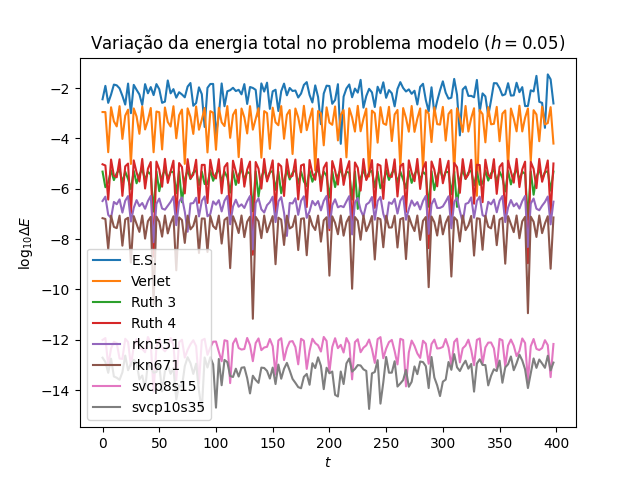
\includegraphics[width=0.7\linewidth]{tcc//img/var_energia_simpleticos.png}
    \caption{Variação da energia total para os métodos simpléticos apresentados. O problema-modelo \ref{probmodelo:lemniscata} foi integrado no intervalo $[0,400]$ com tamanho de passo $h=0.05$.}
    \label{fig:var_energia_simpleticos}
\end{figure}

Um ponto importante sobre os métodos simpléticos é que, como já dito, estes conservam não apenas a energia total, mas todas as integrais primeiras. Porém, a energia total é calculada através das velocidades e das distâncias entre os corpos, e corpos muito próximos geram instabilidade numérica no sentido de facilitarem o aparecimento de erros de ponto flutuante, enquanto as outras quantidades conservadas baseiam-se somente em operações lineares ou vetoriais diretas, sem a possibilidade de singularidades. A implicação prática disso é que as outras integrais primeiras são muito melhor conservadas que a energia total, como pode ser observado na figura \ref{fig:var_integrais_es_iau25}, na qual as outras integrais primeiras de um problema de 25 corpos possuem erro abaixo de $10^{-11}$. Dessa forma, é coerente analisar erros numéricos focando-se principalmente na energia.

\begin{figure}
    \centering
    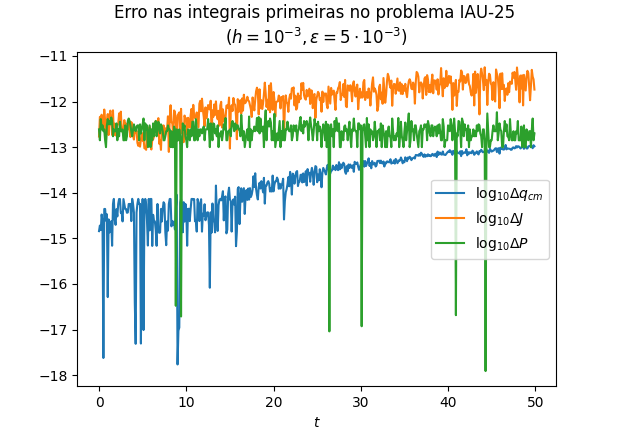
\includegraphics[width=0.5\linewidth]{tcc//img/var_integrais_es_iau25.png}
    \caption{Variação das integrais primeiras do PNCG na simulação do problema IAU-25 (\ref{probmodelo:iau25}) via método de Euler Simplético com tamanho de passo $h=10^{-3}$ e amortecimento $\epsilon=10^{-3}$. Aqui $\Delta f = |\norma{f} - \norma{f_0}|$.}
    \label{fig:var_integrais_es_iau25}
\end{figure}

%%%%%%%%%%%%%%%%%%%%%%%%%%%%%%%%%%%%%%%
%%% CORRETOR NUMÉRICO
%   Falar sobre o corretor numerico e exemplos de sua
%   aplicacao em problemas grandes e pequenos, alem do
%   custo computacional e da eficiencia.
%%%%%%%%%%%%%%%%%%%%%%%%%%%%%%%%%%%%%%%
\section{Corretor numérico}\label{secao:corretor_numerico}

Uma alternativa (ou complemento) ao uso de integradores simpléticos é utilizar integradores tradicionais e aplicar algum tipo de correção a cada passo, de modo a garantir que a solução aproximada conserve as integrais primeiras. O método apresentado nesta seção tem esse propósito, e, embora aqui tenha sido desenvolvido intuitivamente, este foi proposto inicialmente por \cite{Nacozy1972} e posteriormente analisado por \cite{Shampine1986}.

Sejam $\vet z = (\vet q, \vet p)$ um vetor no espaço de fases para um problema de $N$ partículas (não necessariamente o PNCG) e $\vet z_0 = (\vet q_0, \vet p_0)$ o valor inicial de um Problema de Cauchy conservativo
\begin{equation*}
    \dvet z (t) = F(t,\vet z(t)), \quad \vet z(t_0) = \vet z_0,
\end{equation*}
com $F$ suave. Seja também $\vet \Psi (\vet z) = (\psi_1(\vet z), ..., \psi_k(\vet z))$ um conjunto de $k$ integrais primeiras para o problema, sendo $\vet \Psi_0 = \vet \Psi(\vet z_0)$.

Tome um instante $t \in I$, sendo $I$ o intervalo maximal do problema, e considere a solução exata $\vet z^* = \vet z(t)$ e a solução aproximada $\tilde{\vet z}$, obtida através de um integrador numérico qualquer. Espera-se de uma boa simulação conservativa que $\vet z$ seja solução de
\begin{equation}\label{eq:problema_otimizacao_corretor}
    \begin{aligned}
        \min \quad & \norma{\tilde{\vet z} - \vet z^*} \\
        \text{s. a} \quad & \psi_i (\vet z^*) = \psi_i (\vet z_0) \\
        &  i = 1, ..., k.
    \end{aligned}
\end{equation}
Como o que se tem é $\tilde{\vet z}$, podemos analisar em função de $\vet z^*$.

\begin{figure}
    \centering
    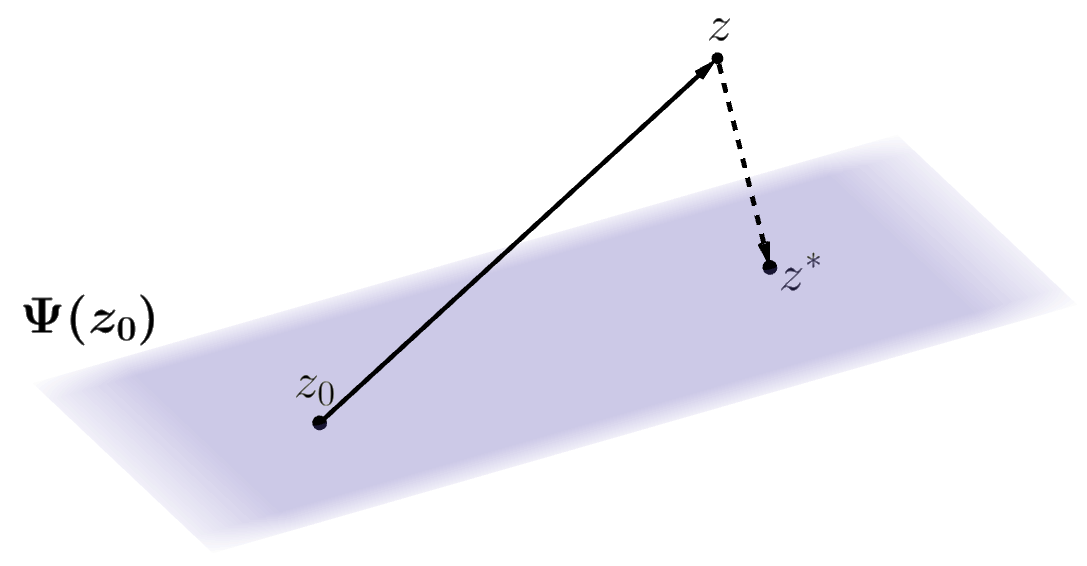
\includegraphics[width=0.5\linewidth]{tcc//img/corretor_visualizacao.png}
    \caption{Representação visual do corretor numérico.}
    \label{fig:corretor_visualizacao}
\end{figure}

Tome uma função $f(\vet x) = \frac{1}{2} \norma{\tilde{\vet z} - \vet x}^2$, cujo problema de otimização é equivalente a (\ref{eq:problema_otimizacao_corretor}). O processo se torna o método de quadrados mínimos. Tome $\vet y$ um candidato a mínimo do problema. As condições necessárias de otimização para o problema implicam que nesse caso \citep{Friedlander1994}:
\begin{equation}\label{eq:corretor_equacao_1}
    \nabla f(\vet y) = \tilde{\vet z} - \vet y
    = \sum_{i=1}^k \alpha_i \nabla \psi_i (\vet y) = D \vet \Psi (\vet y)^T \vet \alpha, 
    \quad \vet \alpha = (\alpha_1, ..., \alpha_k),
\end{equation}
onde $D \vet \Psi (\vet y)$ é a matriz jacobiana do campo vetorial de integrais primeiras e $\vet \alpha$ é o vetor de multiplicadores de Lagrange. Observe que a função objetivo $f$ é uma função convexa, e logo a condição necessária é também suficiente para o problema. Por Taylor, tem-se que
\begin{equation*}
    \vet \Psi (\tilde{\vet z}) \approx \vet \Psi (\vet y) + D \vet \Psi(\vet y) (\tilde{\vet z} - \vet y),
\end{equation*}
o que pela equação (\ref{eq:corretor_equacao_1}) pode ser escrito como:
\begin{equation}\label{eq:corretor_equacao_2}
    D \vet \Psi(\vet y) D \vet \Psi(\vet y)^T \vet \alpha 
    \approx
    \vet \Psi (\tilde{\vet z}) - \vet \Psi(\vet y)
    = 
    \vet \Psi (\tilde{\vet z}) - \vet \Psi(\vet z_0).
\end{equation}

Resolvendo (\ref{eq:corretor_equacao_2}) obtém-se os multiplicadores de Lagrange, que podem ser substituídos em (\ref{eq:corretor_equacao_1}):
\begin{equation*}
    \vet y = \tilde{\vet z} - D \vet \Psi(\vet y)^T \vet \alpha \approx \vet z^*.
\end{equation*}

Dessa forma, ainda que seja utilizado um método tradicional, é possível obter uma solução que preserve \textit{razoavelmente} as integrais primeiras. Essa \textit{razoabilidade} está ligada com o tamanho de passo $h$ escolhido da maneira como segue.

Considere um problema local no instante $t_n$ dado por
\begin{equation*}
    \dvet u (t) = F(t, \vet u(t)), \quad \vet u(t_n) = \vet z_n^*,
\end{equation*}
onde $\vet z_n$ é uma aproximação para o problema original no instante $t_n$ que satisfaz as integrais primeiras. Um tamanho de passo $h$ está relacionado a um erro local $\tau$ de modo que
\begin{equation*}
    \norma{u(t_{n+1}) - \vet z_{n+1}} \leq \tau.
\end{equation*}
Tomando uma aproximação corrigida $\vet z_{n+1}^*$, observe que
\begin{align*}
    \norma{\vet z(t_{n+1}) - \vet z_{n+1}^*} 
    & = \norma{\vet z(t_{n+1}) - \vet u(t_{n+1}) + \vet u(t_{n+1}) - \vet z_{n+1} + \vet z_{n+1} - \vet z_{n+1}^*} \\
    & \leq \norma{\vet z(t_{n+1}) - \vet u(t_{n+1})} + \norma{\vet u(t_{n+1}) - \vet z_{n+1}} + \norma{\vet z_{n+1} - \vet z_{n+1}^*} \\
    & \leq \zeta_h + \tau + \mu,
\end{align*}
onde $\zeta_h$ limita a norma de $\vet z(t_{n+1}) - \vet u(t_{n+1})$ e $\mu = \norma{\vet z_{n+1} - \vet z_{n+1}^*}$. A constante $\zeta_h$ é garantida por $f$ ser Lipschitz com constante $L$:
\begin{equation*}
    \norma{\vet z(t_{n+1}) - \vet u(t_{n+1})} \leq e^{h L} \norma{\vet z(t_n) - \vet z_n^*} = \zeta_h.
\end{equation*}
Quanto à $\mu$, se garantida sua existência como constante, então aplicar a correção sobre uma aproximação com erro $\tau$ possui um erro de discretização equivalente a não aplicar a correção sobre uma aproximação de erro $\tau + \mu$. 

Observe que $\vet u(t)$ satisfaz as integrais primeiras, pois seu valor inicial $\vet z_n^*$ as satisfaz. Em particular $\vet u(t_{n+1}) = \vet z_{n+1}^*$ satisfaz, e logo a correção é tal que $\mu = \tau$, o que significa que aplicá-la sobre uma aproximação de ordem $p$ fornece uma aproximação corrigida também de ordem $p$. Dessa forma, o corretor preserva a ordem do integrador.

Quanto à aplicação computacional, algumas questões merecem ser tratadas, e constam na seção \ref{secao:uso_do_corretor}.